
%%%%%%%%%%%%%%%%%%%%%%%%%%%%%%%%%%%%%%%%%%%%%%%%%%%%%%%%%%%%%%%%%%%%%%%%%%%%
%%%%%%%%%%%%%%%%%%%%%%%%%%%%%%%%%%%%%%%%%%%%%%%%%%%%%%%%%%%%%%%%%%%%%%%%%%%%
%%%%%%%%%%%%%%%%%%%%%%%%%%%%%%%%%%%%%%%%%%%%%%%%%%%%%%%%%%%%%%%%%%%%%%%%%%%%

\begin{frame}[t]{Formalizing the question.}

\begin{minipage}[t]{0.45\textwidth}
\textbf{Ordinary least squares}

\vspace{1em}
A data point $\d_n$ has regressors
$x_n$ and response $y_n$: $\d_n = (x_n, y_n)$.

\vspace{1em}
The estimator $\thetahat \in \mathbb{R}^p$ satisfies:
%
\begin{align*}
%
\thetahat :={}&
    \argmin_{\theta} \frac{1}{2} \sumn \left(y_n - \theta^T x_n \right)^{2} \\
\Leftrightarrow{}& \sumn \left(y_n - \thetahat^T x_n \right) x_n = 0.
%
\end{align*}
%
Make a qualitative decision using:\vspace{-1.5em}
\begin{itemize}
\item A particular component: $\thetahat_k$
\item The end of a confidence interval:
    $\thetahat_k + \frac{1.96}{\sqrt{N}} \hat\sigma(\thetahat)$
\end{itemize}
%
\end{minipage}
%
\hfill\vline\hfill
%
\begin{minipage}[t]{0.45\textwidth}
\textbf{Z-estimators}

\vspace{1em}
We observe $N$ data points $\d_{1}, \ldots, \d_{N}$
(in any domain).

\vspace{1em}
The estimator $\thetahat \in \mathbb{R}^p$ satisfies:
%
\begin{align*}
%
\sumn
G(\thetahat, \d_{n}) =  \zP.
%
\end{align*}
%
$G(\cdot, \d_{n})$ is ``nice,'' $\mathbb{R}^p$-valued.

E.g. OLS, MLE, VB, IV \&c.

\vspace{1em}
Make a qualitative decision using $\thetafun(\thetahat)$
for a smooth, real-valued $\thetafun$.

\vspace{1em}
(WLOG try to increase $\thetafun(\thetahat)$.)
%
\end{minipage}

% \hrulefill

% \vspace{0.3em}
% \textbf{Question: }
% Can we make a big change in $\thetafun(\thetahat)$ by dropping
% $\alphan$ datapoints, for some small proportion $\alpha$?

\end{frame}





%%%%%%%%%%%%%%%%%%%%%%%%%%%%%%%%%%%%%%%%%%%%%%%%%%%%%%%%%%%%%%%%%%%%%%%%%%%%
%%%%%%%%%%%%%%%%%%%%%%%%%%%%%%%%%%%%%%%%%%%%%%%%%%%%%%%%%%%%%%%%%%%%%%%%%%%%
%%%%%%%%%%%%%%%%%%%%%%%%%%%%%%%%%%%%%%%%%%%%%%%%%%%%%%%%%%%%%%%%%%%%%%%%%%%%

\begin{frame}[t]{Data dropping as data reweighting.}

\textbf{Question: }
Can we make a big change in $\thetafun(\thetahat)$ by dropping
$\alphan$ datapoints, for some small proportion $\alpha$?
%
\textbf{Two big problems:}
%
\begin{itemize}
    \item There are ${N \choose \alphan}$
        sets to check.
        (E.g. ${16,560 \choose 15 } \approx 1.5\cdot10^{51}$)
    \item Evaluating $\thetahat$ re-solving the estimating equation.
        \begin{itemize}
        \item E.g., re-computing the OLS estimator.
        \item Other examples are even harder (VB, machine learning)
        \end{itemize}
\end{itemize}
%
\textbf{Our idea: }Smoothly approximate the effect of leaving out points.

\hrulefill

We have $N$ data points $\d_{1}, \ldots, \d_{N}$, a quantity of interest
$\thetafun(\cdot)$, and
%
\begin{align*}
%
\sumn
\only<2->{\color{red} \w_n \color{black}}
G(
\thetahat\only<2->{\color{red} (\w) \color{black}}
, \d_{n}) =  \zP
\onslide<2->{\textrm{ for a weight vector }\w \in \mathbb{R}^N}.
%
\end{align*}

\onslide<3->{
\begin{minipage}{0.45\textwidth}
\begin{center}
Original weights: $\onevec = (1,\ldots,1)$
    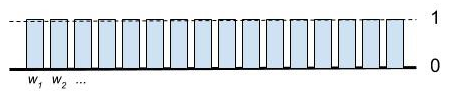
\includegraphics[width=1.0\textwidth]{static_figures/orig_weights}
\end{center}
\end{minipage}
\begin{minipage}{0.45\textwidth}
\begin{center}
Leave points out by setting their elements of $\w$ to zero.
    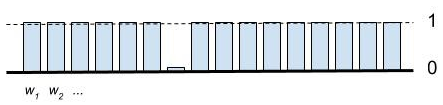
\includegraphics[width=1.0\textwidth]{static_figures/weights_loo}
\end{center}
\end{minipage}
}

\onslide<3->{
The map $\w \mapsto \thetafun(\thetahat(\w))$ is well-defined even
for continuous weights.
}



\end{frame}



%%%%%%%%%%%%%%%%%%%%%%%%%%%%%%%%%%%%%%%%%%%%%%%%%%%%%%%%%%%%%%%%%%%%%%%%%%%%
%%%%%%%%%%%%%%%%%%%%%%%%%%%%%%%%%%%%%%%%%%%%%%%%%%%%%%%%%%%%%%%%%%%%%%%%%%%%
%%%%%%%%%%%%%%%%%%%%%%%%%%%%%%%%%%%%%%%%%%%%%%%%%%%%%%%%%%%%%%%%%%%%%%%%%%%%



\def\LinearGraph{
\begin{center}
    \begin{tikzpicture}
        \node[anchor=south west,inner sep=0] (image) at (0,0) {
            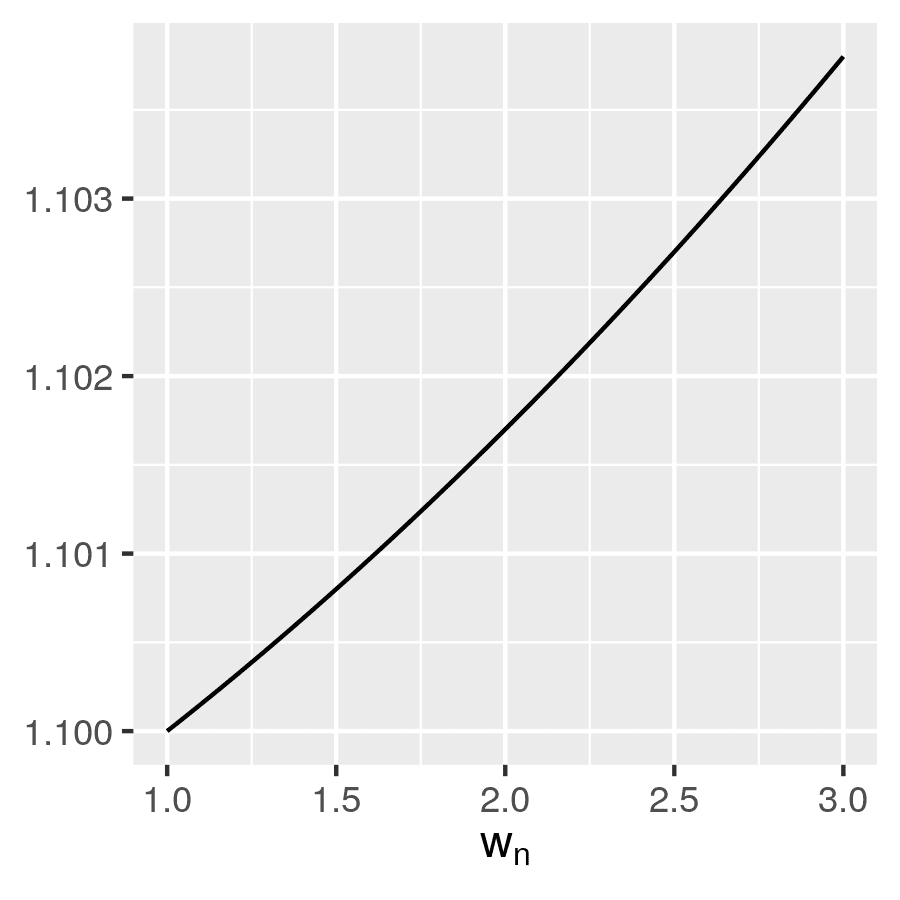
\includegraphics[width=0.78\textwidth]{static_figures/e_beta_w}
        };
        \begin{scope}[x={(image.south east)},y={(image.north west)}]
            \draw[blue, thick, <-] (0.2,0.23) -- ++(0.1,0.25)
                    node[above,black,fill=white]
                    {\small $\thetafun(\thetahat(\onevec))$};
            \draw[blue, thick, <-] (0.8,0.8) -- ++(-0.1,0.1)
                    node[left,black,fill=white]
                    {\small $\thetafun(\thetahat(\w))$};
            \draw[red, thick, -] (0.18,0.18) -- ++(1.2 * 0.6, 1.2 * 0.48);
            \draw[blue, thick, <-] (0.75,0.55) -- ++(0.02,-0.1)
                    node[below right,black,fill=white]
                    {\small Slope $ =
                    \fracat{\partial \thetafun(\thetahat(\w))}
                           {\partial\w_n}{\onevec}
                    =: \infl_n$};
        \end{scope}
    \end{tikzpicture}
\end{center}
}


\begin{frame}[t]{Taylor series approximation.}
\vspace{-2em}
\begin{align*}
%
\sumn \w_n
G(\thetahat(\w), \d_{n}) =  \zP
\textrm{ for a weight vector }\w \in \mathbb{R}^N.
%
\end{align*}
%
% \begin{minipage}{0.45\textwidth}
% \begin{center}
% Original weights: $\onevec = (1,\ldots,1)$
%     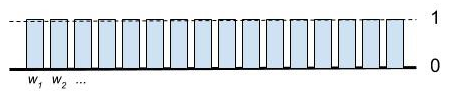
\includegraphics[width=1.0\textwidth]{static_figures/orig_weights}
% Leave points out by setting their elements of $\w$ to zero.
%     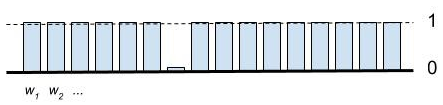
\includegraphics[width=1.0\textwidth]{static_figures/weights_loo}
% \end{center}
% \end{minipage}
\begin{center}
\begin{minipage}{0.45\textwidth}
\LinearGraph{}
\end{minipage}
\end{center}

The values $N \infl_n$ are the \textbf{empirical influence function}
\citep{hampel1986robustbook}.

We call $\infl_n$ an ``influence scores.''

\vspace{1em}
We can use $\infl_n$ to form a Taylor series approximation:
%
\begin{align*}
	\thetafun(\thetahat(\w))
		&\approx
        \color{red}
        \thetafunlin(\w)
        \color{black}
		:=  \thetafun(\thetahat(\onevec)) +
        \sumn \infl_n (\w_n -1)
        \color{black}
\end{align*}

\end{frame}




%%%%%%%%%%%%%%%%%%%%%%%%%%%%%%%%%%%%%%%%%%%%%%%%%%%%%%%%%%%%%%%%%%%%%%%%%%%%
%%%%%%%%%%%%%%%%%%%%%%%%%%%%%%%%%%%%%%%%%%%%%%%%%%%%%%%%%%%%%%%%%%%%%%%%%%%%
%%%%%%%%%%%%%%%%%%%%%%%%%%%%%%%%%%%%%%%%%%%%%%%%%%%%%%%%%%%%%%%%%%%%%%%%%%%%


\begin{frame}{Taylor series approximation.}
%
\textbf{Problem: }
%
How much can you change $\thetafun(\thetahat(\w))$
dropping $\alphan$ points?

\textbf{Combinatorially hard by brute force!}

\hrulefill

\textbf{Approximate Problem: }
%
How much can you change $\thetafunlin(\thetahat(\w))$
dropping $\alphan$ points?
%
\textbf{Easy! }
%
\begin{align*}
    \thetafunlin(\w)
		:=  \thetafun(\thetahat(\onevec)) +
        \sumn \infl_n (\w_n -1)
\end{align*}
%
Dropped points have $\w_n - 1 = -1$.  Kept points have $\w_n - 1 = 0$

$\Rightarrow$ The most influential points for $\thetafunlin(\w)$ have the
most negative $\infl_n$.

\hrulefill

\textbf{Our procedure:}  (see \texttt{rgiordan/zaminfluence} on \texttt{github})
\begin{enumerate}
    \item Compute your original estimator $\thetahat(\onevec)$.
    \item Compute and sort the influence scores
        $\infl_{(1)}, \ldots, \infl_{(N)}$.
    \item Worry if $- \sum_{n=1}^{\alphan} \infl_{(n)}$ is large
    enough to change your conclusions.
\end{enumerate}

How to compute the $\infl_n$'s?  And how accurate is the approximation?

\end{frame}

% %%%%%%%%%%%%%%%%%%%%%%%%%%%%%%%%%%%%%%%%%%%%%%%%%%%%%%%%%%%%%%%%%%%%%%%
% %%%%%%%%%%%%%%%%%%%%%%%%%%%%%%%%%%%%%%%%%%%%%%%%%%%%%%%%%%%%%%%%%%%%%%%
% %%%%%%%%%%%%%%%%%%%%%%%%%%%%%%%%%%%%%%%%%%%%%%%%%%%%%%%%%%%%%%%%%%%%%%%

\begin{frame}[fragile]{How to compute the influence scores?}

How can we compute the influence scores
%
%\begin{align*}
%
$
\infl_n =
\fracat{\partial \thetafun(\thetahat(\w))}
       {\partial\w_n}{\onevec}
%
$?
%\end{align*}
%

\vspace{1em}
By the \textbf{chain rule},
$
\infl_n =
\fracat{\partial \thetafun(\theta)}
      {\partial\theta}{\thetahat(\onevec)}
\fracat{\partial \thetahat(\w)}
    {\partial\w_n}{\onevec}
%
$.

\vspace{1em}
Recall that
$\sumn \w_n G(\thetahat(\w), \d_{n}) =  \zP$ for all $\w$ near $\onevec$.


\vspace{1em}
$\Rightarrow$
By the \textbf{implicit function theorem}, we can write
$\fracat{\partial\thetahat(\w)}{\partial\w_n}{\onevec}$ as a linear system
involving $G(\cdot, \cdot)$ and its derivatives.

\vspace{1em}
$\Rightarrow$
The $\infl_n$ are automatically computable from $\thetahat(\onevec)$ and
software implementations of $G(\cdot, \cdot)$ and $\thetafun(\cdot)$
using \textbf{automatic differentiation}.



\begin{lstlisting}
> import jax
> import jax.numpy as np
> def phi(theta):
>     ... computations using np and theta ...
>     return value
>
> # Exact gradient of phi (first term in the chain rule above):
> jax.grad(phi)(theta_opt)
\end{lstlisting}

See \texttt{rgiordan/vittles} on \texttt{github}.

\end{frame}


% %%%%%%%%%%%%%%%%%%%%%%%%%%%%%%%%%%%%%%%%%%%%%%%%%%%%%%%%%%%%%%%%%%%%%%%
% %%%%%%%%%%%%%%%%%%%%%%%%%%%%%%%%%%%%%%%%%%%%%%%%%%%%%%%%%%%%%%%%%%%%%%%
% %%%%%%%%%%%%%%%%%%%%%%%%%%%%%%%%%%%%%%%%%%%%%%%%%%%%%%%%%%%%%%%%%%%%%%%

\begin{frame}{How accurate is the approximation?}

% Mexico example:

% See \texttt{microcredit\_profit\_sandbox.R}.

\begin{center}
Checking the approximation for Mexico microcredit.
\end{center}

% 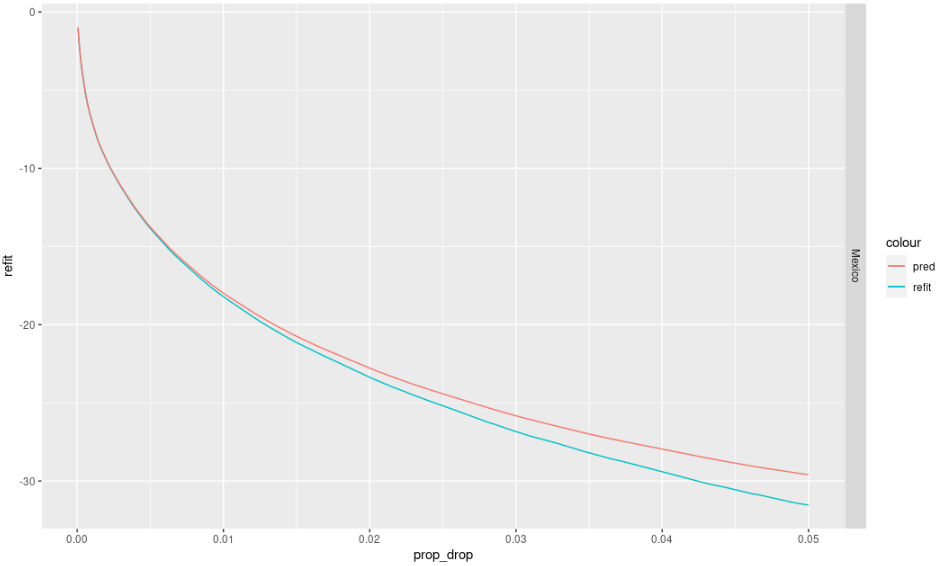
\includegraphics[width=0.9\textwidth]{static_figures/mx_refit_example}
\only<1>{\SimRefitOne{}}
\only<2>{\SimRefitTwo{}}



\end{frame}


% %%%%%%%%%%%%%%%%%%%%%%%%%%%%%%%%%%%%%%%%%%%%%%%%%%%%%%%%%%%%%%%%%%%%%%%
% %%%%%%%%%%%%%%%%%%%%%%%%%%%%%%%%%%%%%%%%%%%%%%%%%%%%%%%%%%%%%%%%%%%%%%%
% %%%%%%%%%%%%%%%%%%%%%%%%%%%%%%%%%%%%%%%%%%%%%%%%%%%%%%%%%%%%%%%%%%%%%%%

\begin{frame}{How accurate is the approximation?}

\begin{minipage}{0.45\textwidth}
    By conrolling the curvature,
    % $\fracat{\partial^2 \thetafun(\thetahat(\w))}
    %         {\partial \w_n \partial \w_m}
    %         {\onevec}$
    we can control the error in the linear approximation.

    % \vspace{1em}
    % Key conditions are
    % \begin{itemize}
    %     \item Smoothness of $\thetafun(\cdot)$,
    %         $\meann G(\cdot, \d_n)$, and derivatives
    %     \item Invertibility of
    %         $\meann \fracat{\partial G(\theta, \d_n)}
    %             {\partial \theta^T}{\thetahat(\onevec)}$.
    % \end{itemize}
\end{minipage}
%
\begin{minipage}{0.45\textwidth}
\LinearGraph{}
\end{minipage}

\vspace{1em}
We provide \textbf{finite-sample theory}
\citep{giordano2019swiss}
showing that
$\abs{\thetafun(\thetahat(\w)) - \thetafunlin(\w)} =
O\left(\vnorm{\frac{1}{N}(\w - \onevec)}^2_2\right) =
O\left(\alpha\right)$ as $\alpha \rightarrow 0$.

\vspace{1em}

\hrulefill

\vspace{1em}
\textbf{But you don't need to rely on the theory!}

\vspace{1em}
Our method returns which points to drop.  \textbf{Re-running once}
without those
points provides an \textbf{exact lower bound} on the worst-case
sensitivity.

\end{frame}
